\newpage
\part{Maximum Lifespan Assessment (MaxLifespan)} \label{part:ap}

\section{Introduction to maxium (best) lifespan mapping} \label{sec:actintro}
The \textit{MaxLifespan} module serves for the GIS -- based prioritization of stream restoration features based on lifespan and design maps and it creates \texttt{raster}s, \texttt{shapefiles}, \texttt{mxd}-layouts and \texttt{pdf}-maps. This chapter is structured as follows:\\
\begin{tabular}{l L{0.9\textwidth}}
\multicolumn{2}{l}{}\\
Section~\ref{sec:actquick}: & Quick Guide to the application of the GUI with description of required input (rasters), alternative run options and output descriptions.\\
Section~\ref{sec:actprin}:  & Descriptions of outputs and procedures for half-automated pdf-map generation.\\
Section~\ref{sec:actcode}:  & Detailed explanations of coding conventions with descriptions of extension possibilities.\\
\multicolumn{2}{l}{}\\
\end{tabular}

Maximum lifespan mapping uses lifespan maps produced with the \textit{LifespanDesign} to identify the feature(s) with the highest lifespan for every pixel within the three feature groups. If the maximum pixel lifespan can be obtained by several features, the \textit{MaxLifespan} module overlays polygons indicating the best feature types. For terrain modifications, all relevant features (grading, widening/berm setback, backwater enhancement as well as side channel or side cavity creation) are equally considered. Thus, the planner has to decide and manually manipulate feature polygons which are relevant for the particular project. Regarding toolbox features, the \textit{MaxLifespan} module evaluates plantings against wood (engineered log jams) and angular boulders (rocks) placement to increase habitat suitability and stabilize terrain modifications. Again the planner has to decide, which plantings, wood or angular boulders (rocks) polygons are relevant to keep for the final version. Finally, the \textit{MaxLifespan} module uses complementary feature lifespan and design maps as well as terrain slope analysis to highlight areas where gravel augmentation, the incorporation of fine sediment in the soil and bioengineering features for terrain/slope stabilization are relevant. Also in this last step, the planner needs to decide, which feature polygons to keep. However, if the analysis of complementary features identifies unstable slopes, it is strongly recommended to take action in the concerned areas.


\section{Quick GUIde to maximum lifespan maps} \label{sec:actquick}
\subsection{Main window set-up and run} 
The \textit{MaxLifespan} module requires lifespan and design maps, i.e., the prior run of the \textit{LifespanDesign} module is required. Then, the \textit{MaxLifespan} module can be launches and Fig.~\ref{fig:gui_start_ap} shows the \textit{MaxLifespan} GUI after the module start-up.\\
First, the module requires the choice of a feature set from the dropdown menu. Second, a \texttt{condition} needs to be defined analog to the \textit{LifespanDesign} module (exactly four characters, see Sec.~\ref{sec:input}).
\begin{figure}[hbt]
	\begin{center}
	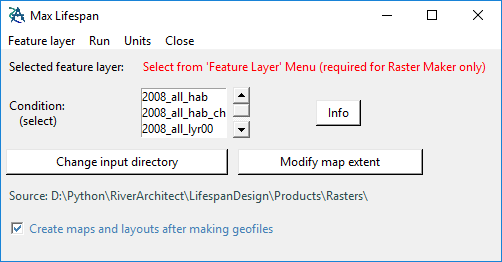
\includegraphics[width=0.7\columnwidth]{gui_start_ap.PNG} % Example image
	\caption{GUI start up window. \label{fig:gui_start_ap}}
	\end{center}
\end{figure}

By default, the \textit{MaxLifespan} will look up lifespan and design maps that are stored in the folder \texttt{.../RiverArchi tect/LifespanDesign/Products/Rasters/\textit{condition}/}. This input directory can be modified by clicking on the \texttt{Change input directory} button. Furthermore, the extents of the maximum lifespan map output can be modified by clicking on the ``Modify map extent'' button, which opens an input file (\texttt{*.inp}) analog to the \textit{LifespanDesign} module (Sec.~\ref{sec:inpmaps}).\\
The \textit{MaxLifespan} will automatically look for raster files beginning with ``\texttt{lf}'' or ``\texttt{ds}'' and containing the shortname of the considered features (see shortname list in Sec.~\ref{sec:featoverview}. Please note that raster names that do not start with either ``\texttt{lf}'' or ``\texttt{ds}'' and/or that do not contain the complete shortname of the considered features are not recognized by \textit{MaxLifespan}. The background image of the maximum lifespan maps also refers to lifespan and design maps and corresponds to the raster \texttt{.../RiverArchitect/01{\myUnderscore}Conditions/\textit{condition}/back}.\\

The mapping check box provides the optional creation of maps with the creation of geofiles (rasters and shapefiles). If the check box is selected, running the Geofile Maker also includes the successive runs of the Layout Maker and Map Maker. It is recommended to keep this box checked (default) because maximum lifespan mapping is fully automated and the procedure is fast.\\

Once all inputs are defined, click on ``Run'' and ``Verify settings'' to ensure the consistency of the chosen settings. After successful verification, the selected feature list and the verified condition change to green font.\\

Three ``Run'' options exist in the drop-down menu:
\begin{itemize}
\item \pythoninline{Run: Geofile Maker} prepares the optimum lifespan raster and associated feature polygons (shapefiles) in the directories \texttt{RiverArchitect/MaxLifespan/Output/Rasters/\textit{condition}/} and \texttt{.../Output /Shapefiles/\textit{condition}/}
\item \pythoninline{Run: Layout Maker} prepares \texttt{.mxd} layouts in the directory \texttt{RiverArchitect/MaxLifespan/Output/Layout/\textit{condition}/} (more information on layouts in Sec.~\ref{sec:actoutmaps}).
\item \pythoninline{Run: Map Maker} prepares maximum lifespan map assemblies (\texttt{pdf}s) in the directory \texttt{RiverArchitect/MaxLife span/Output/Maps/\textit{condition}/} (more information on layouts in Sec.~\ref{sec:actoutmaps})
\end{itemize}



\subsection{Alternative run options}
\label{sec:actrun}
The three principal run options of the GUI call the following methods:
\begin{enumerate}
\item Run: Geofile Maker calls \pythoninline{action_planner.geo_file_maker} 
\item Run: Layout Maker calls \pythoninline{action_planner.layout_maker} 
\item Run: Map Maker calls \pythoninline{action_planner.map_maker} 
\end{enumerate}

In the batch processing of multiple scenarios, it can be useful to call the \pythoninline{geo_file_maker} from a script as a standalone. This can be done as follows:

\begin{enumerate}
	\item Go to ArcGIS Python folder\\
	Example: \texttt{C:/Python27/ArcGISx64XX.X}
	\item Launch \texttt{python.exe}
	\item Enter \pythoninline{import os}
	\item Navigate to Script direction using the command \pythoninline{os.chdir("ScriptDirectory")}\\
	Example: \pythoninline{os.chdir("D:/Python/RiverArchitect/MaxLifespan/")}
	\item Import the module: \pythoninline{import action_planner as ap}\\
	\item Launch Geofile Maker: \pythoninline{ap.geo_file_maker(condition, feature_type, *args)}, where \pythoninline{args[0]} is a boolean value for activating or deactivation of integrated PDF-mapping (default = False), \pythoninline{args[1]} is a string that indicates the unit system (either ``us'' or ``si''; default = ``us'') and \pythoninline{args[2]} can be an alternative input path of lifespan maps than the default directory (see above)\\
	Example: \pythoninline{ap.geo_file_maker(2008, "framework", True, "us", "D:/temp/")}\\
	This command calls the Geofile Maker for the condition ``2008'' for framework features, with activated mapping, U.S. customary units and it sets the raster input path to \texttt{D:/temp/}.
\end{enumerate}



%----------------------------------------------------------------------------------------
\subsection{Output}
\label{sec:actoutput}
\subsubsection{Geofiles}
The principal output of the module's Geofile Maker is one raster called \texttt{max{\myUnderscore}lf} (stored in \texttt{.../MaxLifespan/Output/Rasters/\textit{condition}/}) and one shapefile per analyzed feature containing polygons of the feature's best performing areas (stored in \texttt{.../MaxLifespan/Output/Shapefiles/\textit{condition}/}). Moreover, the module produces rasters with names corresponding to the lifespan/design raster names and feature shortnames, which essentially contain the same information as the feature shapefiles. These raster files are side products from the production of the feature shapefiles.

\subsubsection{Layouts and Maps} \label{sec:actoutmaps}
The Layout Maker uses \texttt{.mxd} layout templates to overlay
\begin{itemize}
	\item a background raster (\texttt{.../RiverArchitect/01{\myUnderscore}Conditions/\textit{condition}/back}),
	\item the best lifespan raster (\texttt{.../MaxLifespan/Output/Rasters/\textit{condition}/max{\myUnderscore}lf}) and
	\item shapefiles of best performing feature areas (\texttt{.../MaxLifespan/Output/Shapefile/\textit{condition}/lf{\myUnderscore}feat...} or\texttt{ds{\myUnderscore}feat...}).
\end{itemize}

The layouts templates are stored in \texttt{.../MaxLifespan/.templates/layouts/} and they are named after the feature set type; notably \texttt{framework.mxd}, \texttt{toolbox.mxd} and \texttt{complementary.mxd}. These templates can be changed to modify the maximum lifespan map layout, e.g., the legend, paper size, symbology or background source image. Apart from the background image raster, the shapefile and raster sources in the template \texttt{mxd}s refer to the \textit{MaxLifespan}s output folder and the sources should not be modified. The Layout Maker chooses the correct layout as a function of the feature set type and copies this layout to the \texttt{.../MaxLifespan/Output/Layouts/\textit{condition}/} directory.\\

The \textit{MaxLifespan}'s Map Maker run-routine uses this layout copy (\texttt{.mxd}) and the map extent definitions (Sec.~\ref{sec:actquick} and details in Sec.~\ref{sec:inpmaps}). Unlike in the \textit{LifespanDesign} module, the production of maximum lifespan map \texttt{PDF}s completely automated and they are produced in \texttt{.../MaxLifespan/Output/Maps/\textit{condition}/}.\\

The module enforces overwriting of existing files in the output folder and it tries to delete any existing content. Therefore, it is recommended to copy relevant outputs to the directory \texttt{.../MaxLifespan/Products/.../...}.

\subsection{Quit module and logfiles}
The GUI can be closed via the \texttt{Close} dropdown menu if no background processes are going on (see terminal messages). The GUI flashes and rings a system bell when it completed a run task. If layout creation and/or mapping were successfully applied, the target folder automatically opens. After execution of either run task, the GUI disables functionalities, which would overwrite the results and it changes button functionality to open logfiles and quit the program. Logfiles are stored in the \texttt{RiverArchitect/MaxLifespan/} folder and named \texttt{action{\myUnderscore}planner.log}. Logfiles from the previous runs are overwritten.

%----------------------------------------------------------------------------------------

\section{Working principle}\label{sec:actprin}

The Geofile Maker uses the \pythoninline{CellStatistics} (with ``Max'' argument) command of \pythoninline{arcpy}'s Spatial Analyst toolbox to identify the best lifespans of features. In the case of features where only design rasters are available, i.e., raster units are either on/off (1/0) or dimensional indicators (e.g., minimum grain sizes), the Geofile Maker converts any non-zero value of the design raster to 0.8. The value of 0.8 is an arbitrarily chosen identifier with the hypothetical unit of years, where the only importance is that this identifier is larger than zero and smaller than 0.9. Thus, the identifier is smaller than any lifespan value and the \pythoninline{CellStatistic}'s ``Max'' corresponds to the lifespan value when lifespan rasters are compared with design rasters. In other words, the Geofile Maker prioritizes lifespan rasters over design rasters. This choice was made because the data quality of lifespan rasters is better (higher data abundance) than the quality of design rasters, considering that the data quality is a function of available layers (DEM, morphological unit, grain size, hydraulic rasters, etc.). Therefore, pixels where no lifespan value but a design value is available to get assigned a value of 0.8. Finally, the 0.8-pixels are converted to lifespans of 20 years based on the assumption that if the feature is constructed corresponding to the design criteria, its lifespan will be high. Note the difference: lifespan values are prioritized because of the better data quality and the 20-years-value of design raster-only pixels applies to a chain of safe constructive assumptions potentially resulting in high costs.\\

Recall that \texttt{Other bioengineering} features can take three values: (1) \texttt{20.0} years, if the terrain slope is greater than defined in the thresholds workbook and the depth to groundwater is lower than defined in the thresholds workbook (cf. Sec.~\ref{sec:modthresh}); (2) \texttt{1.0} year, if the terrain slope is greater than defined in the thresholds workbook and the depth to groundwater is greater than defined in the thresholds workbook; (3) \texttt{NoData}, if the terrain slope is lower than defined in the thresholds workbook. Thus, where maximum lifespan maps indicate a 1.0-year lifespan, bioengineering features that are independent of the depth to the groundwater table are required. Such features typically imply the placement of angular boulders.



\section{Code modification: Add feature sets for maximum lifespan maps} \label{sec:actcode}
The comprehensive \textit{MaxLifespan} module provides flexibility regarding input directories, layout modifications and mapping extents without modifications of the code. However, modification of the feature sets (framework, toolbox and complementary) require code modifications. The relevant python classes are in the file \texttt{cFeatureActions.py}, notably \pythoninline{class FrameworkFeatures(Director)}, \pythoninline{class ToolboxFeatures(Director)} and \pythoninline{class ComplementaryFeatures(Director)}. These classes all inherit from the \pythoninline{Director} class which identifies and assigns lifespan and design rasters in the input folder. The following code example indicates where single features can be added or removed from feature sets. It is a generalized code sample where ``Framework'', ``Toolbox'' and ``Complementary'' are replaced with ``TYPE''. The feature \pythoninline{FullName_i} and \pythoninline{shortame_i} must comply with the terminology in Sec.~\ref{sec:featoverview} because also the \textit{MaxLifespan} module uses a centralized feature identifier class that is stored in \texttt{RiverArchitect/ModifyTerrain/cDefinitions.py}.\\

\begin{python}
class TYPEFeatures(Director):
    # This class stores all information about TYPE features
    def __init__(self, condition, *args):
        try:
            ## check if args[0] = alternative input path exists
            Director.__init__(self, condition, args[0])
        except:
            Director.__init__(self, condition)
        self.names = ["FullName_1", "FullName_2", ..., "FullName_n"] #--CHANGE HERE
        self.shortnames = ["shortname_1", "shortname_2", ..., "shortname_n"] #--CHANGE HERE
        self.ds_rasters = self.append_ds_rasters(self.shortnames)
        self.lf_rasters = self.append_lf_rasters(self.shortnames)
\end{python}

Moreover, the \pythoninline{choose_ref_layout(self, feature_type)} function of the \pythoninline{Mapper} class in \texttt{MaxLifespan/cMap Actions.py} needs to be updated:
\begin{python}
  def choose_ref_layout(self, feature_type):
    ## type(feature_type) == str
    if type(feature_type) == str:
      if feature_type == "framework":
        ref_layout_name = "framework.mxd"
      if feature_type == "toolbox":
        ref_layout_name = "toolbox.mxd"
      if feature_type == "complementary":
        ref_layout_name = "complementary.mxd"
      if feature_type == "NEW":
        ref_layout_name = "NEW.mxd"
    ...
\end{python}

This also requires the creation of the \texttt{NEW.mxd} layout in \texttt{MaxLifespan/.templates/layouts}.
